\section{Generalization of Lemma~\ref{lem:towerbound_signature}}
\label{app:tower-lemma}
		
%	The generalization of Lemma~\ref{lem:towerbound_signature} is the following: 
	\begin{restatable}{lemma}{lemShortLocalRuns}
	\label{lem:short-local-runs}
		There exists a primitive recursive function $\towerfun$ such that, for every protocol $\prot$ with $r$ registers per agent, 
		for every "local runs" $\localrun_0: (q_0, \localdata_0) \step{*} (q, \localdata)$, $\localrun: (q, \localdata) \step{*} (q', \localdata')$, $\localrun_f: (q', \localdata') \step{*} (q_f, \localdata_f)$, there exists a "local run" $\localrun': (q, \localdata) \step{*} (q', \localdata')$ with $\size{\localrun'} \leq \towerfun(\size{\prot} ,r)$ and for all $\aval' \in \nats$: 
		\begin{enumerate}
			\item if $\aval'$ appears in $\localrun_0$, $\localrun$, or $\localrun_{f}$, $\vinput{\aval'}{\localrun'} \subword \vinput{\aval'}{\localrun}$,
			\item  otherwise, there exists $\aval \in \nats$ such that $\aval$ is not "initial" in $u_0$ and $\vinput{\aval'}{\localrun'} \subword \vinput{\aval}{\localrun}$.
		\end{enumerate}
	\end{restatable}
	The function $\towerfun$ is actually not the same as in Lemma~\ref{lem:towerbound_signature} although it is also a tower of exponentials.
	
	We start by defining the notion of "trace". 
	\AP A ""trace"" is a sequence in $(\set{\extlabel{\atrans}{\aval} \mid \atrans \in \transitions, \aval \in \nats} \cup \set{\intlabel{\atrans} \mid \atrans \in \transitions})^*$. The "trace" of a "local run" $\localrun$ is the "trace" $\trace{\localrun}$ corresponding to the "local steps" performed in $\localrun$. Given a "trace" $\atrace$, we write $(q,\localdata) \step{\atrace} (q',\localdata')$ when there exists a "local run" of "trace" $\atrace$ from $(q,\localdata)$ to $(q',\localdata')$. 
	
	

%We prove the following result:
%\begin{restatable}{lemma}{lemShortLocalRuns}
%	\label{lem:short-local-runs}
%	There exists a primitive recursive function $\towerfun(n,r)$ such that, for every "protocol" with $r$ registers, for every local run $\localrun: (q,\localdata) \step{*} (q', \localdata')$, there exists $u' : (q,\localdata) \step{*} (q',\localdata')$ such that $\size{u'} < \towerfun(\size{\prot},r)$ and for all value $v \in \nats$,  $\vinput{v}{u'} \subword \vinput{v}{u}$. 
%	%	\\
%	%	
%	%	There exists a primitive recursive function $\towerfun(n,r)$ such that, for every protocol $\prot$ with $r$ registers, for every "local run" $\localrun_0: (q_0, \localdata_0) \step{*} (q_f, \localdata_f)$ in $\prot$, for every section $\localrun : (q, \localdata) \step{*} (q, \localdata')$ of $\localrun_0$,  for every $V \subseteq \nats$ finite such that $V$ contains all message values appearing in $\localrun$, there exists a "local run" $\localrun': (q, \localdata) \step{*} (q', \localdata')$ such that we have $\length{\localrun''} \leq \towerfun(\size{\prot},r)$ and:
%	%	\begin{enumerate}
%		%		\item for all $\aval' \in \nats \setminus V$, there exists $\aval$ a "non-initial" value of $\localrun_0$ such that $\vinput{\aval'}{\localrun'}\subword \vinput{\aval}{\localrun}$,
%		%		\item for all $\aval \in V$, $\vinput{\aval}{\localrun'} \subword \vinput{\aval}{\localrun}$. 
%		%	\end{enumerate}
%\end{restatable}


%\lemShortLocalRuns*

We actually prove a more general version of the lemma. The previous lemma can be obtained simply by applying the following one with $W$ the set of "initial" values of $\localrun_0$ ($W$ then contains $r$ values) and $V$ the set of values appearing in $u_0$, $u$ or $u_f$.

\begin{lemma}
	There exists a primitive recursive function $\towerfun(n,r)$ such that, for every protocol $\prot$ with $r$ registers per agent, for every "local run" $\localrun: (q, \localdata) \step{*} (q', \localdata')$ in $\prot$, for every $V \subseteq \nats$ finite such that $V$ contains all message values appearing in $\localrun$,  for every $\Vinit \subseteq V$, there exists a "local run" $\localrun': (q, \localdata) \step{*} (q', \localdata')$ such that we have $\length{\localrun'} \leq \towerfun(\size{\prot} -r + \size{\Vinit},r)$ and:
	\begin{enumerate}
		\item \label{item:shorterrun_oldvalues} for all $\aval \in V$, $\vinput{\aval}{\localrun'} \subword \vinput{\aval}{\localrun}$,
		
		\item \label{item:shorterrun_anyvalue} for all $\aval' \in \nats \setminus V$, there exists $\aval \in \nats \setminus \Vinit$ such that $\vinput{\aval'}{\localrun'} \subword \vinput{\aval}{\localrun}$.
	\end{enumerate}
\end{lemma}

Intuitively, the set $V$ represents values that are already used and therefore cannot be used as fresh values, and $\Vinit$ represents values that should not be copied (\emph{e.g.}, initial values of the run). However, stating the lemma only with $\Vinit$ equal to the initial values in $u$ would not allow us to apply the lemma on $u$ an infix "local run" of a larger "local run" $u'$, because the initial values in $u$ would not correspond to the ones in $u'$. This is why we state the lemma for every $W \subseteq V$.  

\begin{figure}[h]
	

	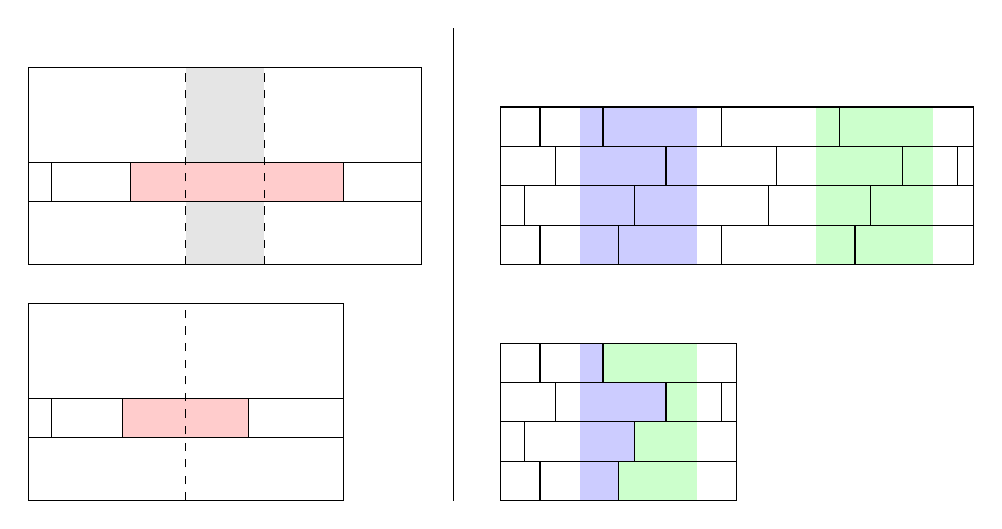
\begin{tikzpicture}
		\draw[white,fill=gray!20] (2,0) rectangle (3,0.8);
		\draw[white,fill=gray!20] (2,1.3) rectangle (3,2.5);
		
		\draw (0,0) rectangle (5,2.5);
		
		\draw (0,0.8) rectangle (5,1.3);
		
		\draw (0,0.8) rectangle (0.3,1.3);
		\draw (0,0.8) rectangle (1.3,1.3);
		\draw[fill=red!20] (1.3,0.8) rectangle (4,1.3);
		
		\draw[dashed] (2,0) -- (2,2.5);
		\draw[dashed] (3,0) -- (3,2.5);
		
		
		
		\draw (0,-3) rectangle (4,-0.5);
		
		\draw (0,-2.2) rectangle (4,-1.7);
		
		\draw (0,-2.2) rectangle (0.3,-1.7);
		\draw (0.3,-2.2) rectangle (1.3,-1.7);
		\draw[fill=red!20] (1.2,-2.2) rectangle (2.8,-1.7);
		
		\draw[dashed] (2,-3) -- (2,-0.5);
		
		\draw (5.4,-3) -- (5.4,3);
		
		
		\draw[white,fill=blue!20] (7,0) rectangle (8.5,2);
		\draw[white,fill=green!20] (10,0) rectangle (11.5,2);
		
		\draw (6,0) rectangle (12,2);
		
		\draw (6,0) rectangle (12,0.5);
		\draw (6,0) rectangle (12,1);
		\draw (6,0) rectangle (12,1.5);
		
		\draw (6,0) rectangle (6.5,0.5);
		\draw (6,0) rectangle (7.5,0.5);
		\draw (6,0) rectangle (8.8,0.5);
		\draw (6,0) rectangle (10.5,0.5);
		
		\draw (6,0.5) rectangle (6.3,1);
		\draw (6,0.5) rectangle (7.7,1);
		\draw (6,0.5) rectangle (9.4,1);
		\draw (6,0.5) rectangle (10.7,1);
		
		\draw (6,1) rectangle (6.7,1.5);
		\draw (6,1) rectangle (8.1,1.5);
		\draw (6,1) rectangle (9.5,1.5);
		\draw (6,1) rectangle (11.1,1.5);
		\draw (6,1) rectangle (11.8,1.5);
		
		\draw (6,1.5) rectangle (6.5,2);
		\draw (6,1.5) rectangle (7.3,2);
		\draw (6,1.5) rectangle (8.8,2);
		\draw (6,1.5) rectangle (10.3,2);
		
		
		\draw[white, fill=blue!20] (7,-3) rectangle (7.5,-2.5);
		\draw[white,fill=blue!20] (7,-2.5) rectangle (7.7,-2);
		\draw[white,fill=blue!20] (7,-2) rectangle (8.1,-1.5);
		\draw[white,fill=blue!20] (7,-1.5) rectangle (7.3,-1);
		
		\draw[white,fill=green!20] (7.5,-3) rectangle (8.5,-2.5);
		\draw[white,fill=green!20] (7.7,-2.5) rectangle (8.5,-2);
		\draw[white,fill=green!20] (8.1,-2) rectangle (8.5,-1.5);
		\draw[white,fill=green!20] (7.3,-1.5) rectangle (8.5,-1);
		
		
		
		\draw (6,-3) rectangle (9,-2.5);
		\draw (6,-3) rectangle (9,-2);
		\draw (6,-3) rectangle (9,-1.5);
		\draw (6,-3) rectangle (9,-1);
		
		\draw (6,-3) rectangle (6.5,-2.5);
		\draw (6,-3) rectangle (7.5,-2.5);
		
		\draw (6,-2.5) rectangle (6.3,-2);
		\draw (6,-2.5) rectangle (7.7,-2);
		
		\draw (6,-2) rectangle (6.7,-1.5);
		\draw (6,-2) rectangle (8.1,-1.5);
		\draw (6,-2) rectangle (8.8,-1.5);
		
		\draw (6,-1.5) rectangle (6.5,-1);
		\draw (6,-1.5) rectangle (7.3,-1);
		
	\end{tikzpicture}


	\caption{Illustration of the proof of Lemma~\ref{lem:short-local-runs}. $s \in \transitions^{2M}$ corresponds to the repeating sequence of transitions of length $2M$. Register $4$ contains value $v \in W$. Because both sides have the same $\Theta$, they coincide on values in $W$ such as $v$; only values that are not in $W$ are replaced by fresh values, hence $v$ is kept in the shortened local run.}
	\label{fig:pumping}
\end{figure}

\begin{proof}
	Given a "local run" $\localrun$, register $i$ is ""active"" in $\localrun$ if at least one $\quotemarks{\enregact}$ step on register $i$ is performed in $\localrun$. 
	
	We define the function $\towerfun(n,k)$ recursively as $\towerfun(n,0) = n+1$ and $\towerfun(n,k+1) = 2(\towerfun(n,k) +1) [(n+1)^{4(\towerfun(n,k)+1)} +1]$. This function is clearly primitive recursive, although non-elementary; it grows as a tower of exponentials of height $k$ where each floor of the tower is polynomial in $n$.
	% A straightforward induction allows one to bound (roughly) $\towerfun(n)(k)$ between the towers of exponentials
	% $n^{n^{{\scriptstyle\cdot^{\scriptstyle\cdot^{\scriptstyle\cdot^{\scriptstyle n}}}}}}$ and $(4n^8+2)^{(4n^8+2)^{\scriptstyle {~\cdot^{\scriptstyle~\cdot^{\scriptstyle~\cdot^{\scriptstyle (4n^8+2)}}}}}}$  of height $k+1$.
	
	We prove the ""shortening property"": \\
	Let $W$ a finite set a values and $n:=\size{\prot} -r + \size{\Vinit}$.
	Let a "local run" $\localrun: (q_i, \localdata_i) \step{*} (q_f, \localdata_f)$ with $k$ "active registers" with $\length{\localrun} > \towerfun(n,k)$ and let $V \subseteq \nats$ finite that contains every message value appearing in $\localrun$ such that $W \subseteq V$. We claim that $\localrun$ can be shortened into a local run $\localrun': (q_i, \localdata_i) \step{*} (q_f, \localdata_f)$ with $k$ active registers such that $\length{\localrun'} < \length{\localrun}$ and:
	\begin{itemize}
		\item for all $\aval \in V$, $\vinput{\aval}{\localrun'} \subword \vinput{\aval}{\localrun}$,
		\item for all $\aval' \in \nats \setminus V$, there exists $\aval \in \nats \setminus W$ such that $\vinput{\aval'}{\localrun'}$ is a subword of $\vinput{\aval}{\localrun}$.
	\end{itemize}
	
	We proceed by induction on the number $k$ of "active registers" in the "local run". If $k=0$, register values do not change in $\localrun$. As $\towerfun(n,0) = n+1 \geq \size{Q}+1$, $\localrun$ goes through the same state twice, hence all steps in between may be removed to get $\localrun'$. Then for all $v \in \nats$,  $\vinput{\aval}{\localrun'} \subword \vinput{\aval}{\localrun}$.
	
	Suppose that the property is true for any "local run" with $\leq k$ "active registers", and consider one $\localrun: (q_i,\localdata_i) \step{*} (q_f,\localdata_f)$ with $k+1$ "active registers" such that $\length{\localrun} > \towerfun(\size{\prot} -r + \size{\Vinit},k+1)$. 
	
	
	First, if there exists an infix "local run" $\localrun_i$ of $\localrun$ of length $\towerfun(n,k)+1$ with only $k$ active registers, then it suffices to apply the induction hypothesis on $u_i$.
	Suppose now that there exists no such infix "local run".
	Let $I \subseteq \nset{1}{r}$ the set of "active registers" in $\localrun$, $|I| = k+1$. Let $M:= \towerfun(n,k){+}1$, we have $\towerfun(n,k+1) = 2M [((n+1)^2)^{2M}+1]$. 
	In any sequence of $M$ "local steps" in a row in $\localrun$, 
	there is a $\quotemarks{\enregact}$ transition on every register in $I$. We can assume that  no local configuration appears twice in $\localrun$ (otherwise we can simply cut the steps between those two appearances to get $\localrun'$). 
	
	In what follows we will consider two infixes of $\localrun$ of length $2M$, following the same sequence of transitions and with the same values of $W$ appearing at the same times in the same registers. Their existence is guaranteed by the length of $\localrun$. As a $\quotemarks{\enregact}$ action is performed twice on each register in those two infixes, we will be able to reduce the run as in \cref{fig:pumping}.
	
	For every $i$, let $\atrans_i$ the $i$-th transition in $\localrun$, and let $\theta_i\in \Vinit \cup \set{\bot}$ be such that 
	\[
	\theta_i = 
	\begin{cases}
		& 	v \text{ if the $i$th step of $u$ is a "reception step" $\extlabel{\delta_i}{v}$ with $v \in \Vinit$ } \\ 
		& 	\bot \text{ otherwise}
	\end{cases}
	\]

	For every $i \in \nset{0}{(n+1)^{4M}}$, we write $s_i$ the sequence $\delta_{2  M \cdot i+1}, \delta_{2  M \cdot i+2}, \cdots, \delta_{2 M \cdot i+2M}$ and $\Theta_i$ the sequence $\theta_{2  M \cdot i}, \theta_{2 M \cdot i+1}, \cdots, \theta_{2 M \cdot i+2M}$.
	There are $|\transitions|^{2M}$ possible sequences for $s_i$ and $[\size{\Vinit} +1]^{2M}$ possible sequences for $\Theta_i$.
	By the pigeonhole principle there exist two indices $i_a, i_b$ such that the sequences $s_{i_a}$ and $s_{i_b}$ are equal and also the sequences $\Theta_{i_a}$ and $\Theta_{i_b}$ are equal (as $|\transitions| (\size{\Vinit}+1) \leq (n+1)^2$ because $n=\size{\prot} -r + \size{\Vinit}$). 
	There exist two infix "local runs" $\localrun_a: (q_1, \localdata_1) \step{*} (q_2, \localdata_2)$, $\localrun_b: (q_3, \localdata_3) \step{*} (q_4, \localdata_4)$ in $\localrun$ such that $(q_2,\localdata_2)$ appears strictly before $(q_3,\localdata_3)$ in $\localrun$ and $\localrun_a$ and $\localrun_b$ both have the same sequences of transitions, which we call $s$, and of receptions of values from $\Vinit$, which we call $\Theta$.
	
	Although $\localrun_a$ and $\localrun_b$ have the same sequence of transitions, their "traces" may differ because their "reception steps" may have different values.
	We build a "trace" $\atrace$ such that $(q_1,\localdata_1) \step{\atrace} (q_4, \localdata_4)$ where the underlying sequence of transitions of $\atrace$ is $s$ and the receptions of values of $\Vinit$ match $\Theta$.
	
	For every active register $i \in I$, let $e_i \in \nset{1}{2M}$ denote the index of the first $\quotemarks{\enregact}$ on register $i$ in $s$ and $f_i \in \nset{1}{2M}$ the index of the last $\quotemarks{\enregact}$ on register $i$ in $s$. By hypothesis, because $s$ is of length $2M$, it contains at least two $\quotemarks{\enregact}$ on register $i$, one in the first half and one in the second half, hence $e_i \leq M < M +1 \leq f_i$. 
	
	For every $j \in \nset{1}{2M}$, let $\delta_j$ denote the $j$-th transition of $s$. First, if  $\delta_j$ is a "broadcast", we define the $j$-th "local step" of $\atrace$ as $\intlabel{\delta_j}$. 
	Suppose now that $\delta_j$ is a "reception" of the form $\rec{\amessage}{i}{\anact}$. The $j$-th "local step" of $\localrun_a$ (resp. $\localrun_b$) has underlying transition $\delta_j$ hence is a "reception step" of the form $\extlabel{\delta_j}{\aval_a}$ for some $\aval_a \in V$ (resp. $\extlabel{\delta_j}{\aval_b}$ for some $\aval_b \in V$).
	Because $V$ is finite and $\Vinit \subseteq V$, there exists an injective function $\phi: V \rightarrow \nats$ such that for all $v \in \Vinit$, $\phi(v) = v$ and for all $v \notin \Vinit$, $\phi(v) \notin V$.
	We define the $j$-th "local step" of $\atrace$ to be $\extlabel{\delta_j}{\aval}$ where:
	\begin{itemize}
		\item if $i \notin I$ then its value stays the same throughout $\localrun$, then we set $\aval = \aval_a (= \aval_b)$ 
		\item if $i \in I$ then  
		\begin{itemize}
			\item if $j < e_i$, $\aval = \aval_a$,
			\item if $e_i \leq j < f_i$, $\aval = \phi(\aval_a)$,
			\item if $f_i \leq j$, $\aval = \aval_b$.
		\end{itemize}
	\end{itemize}
	We now claim that $(q_1,\localdata_1) \step{\atrace} (q_4,\localdata_4)$. 
	First, for every active register $i$, the last $\quotemarks{\enregact}$ step on register $i$ has value $\localdata_4(i)$ in $\atrace$ (as we are in the case $f_i \leq j$). Hence if every "local step" is valid then the final "local configuration" is $(q_4, \localdata_4)$.
	For every $l \in \nset{0}{2M}$, let $\atrace_l$ denote the prefix of $\atrace$ of length $l$.
	We prove by induction on $l$ that $\atrace_l$ is valid from $(q_1, \localdata_1)$. It is trivially true for $l =0$. Assume that we have $(q_1, \localdata_1) \step{\atrace_l} (q, \localdata)$ and let $\locallabel$ such that $\atrace_l \cdot \locallabel = \atrace_{l+1}$. Let $\atrans$ the underlying transition of $\locallabel$.
	First, $q$ is the initial state of $\atrans$ because $\locallabel$ is valid at step $l+1$ of $\localrun_a$ (and $\localrun_b$). Hence if $\atrans$ is a "broadcast" then $\locallabel$ is valid from $(q,\localdata)$. Suppose now that $\locallabel$ is a "reception step"; let $\atrans =: \rec{m}{i}{\alpha}$.
	Let $\aval_a$, $\aval_b$ be the value of $\locallabel$ in $\localrun_a$ and $\localrun_b$ respectively.

	Let $\localdata_a, \localdata_b$ be the content of registers after the $l$-th step in $\localrun_a$ and $\localrun_b$ respectively. 
	 If $i \notin I$ then $\alpha$ is either $\quotemarks{\dummyact}$ or a test, which is valid as  $\localdata(i) = \localdata_a(i) = \localdata_b(i)$ (value of register $i$ does not change in $u$).	
	Suppose now that $i \in I$, the only problematic case is the one of tests, \emph{i.e.}, $\anact \in \set{\quotemarks{\diseqtestact},\quotemarks{\eqtestact}}$. 
	In this case, we prove that $\binrel{\aval}{\anact}{\localdata(i)}$. First, because the corresponding step is valid in $\localrun_a$ and $\localrun_b$, we have $\binrel{\localdata_a(i)}{\anact}{\aval_a}$ and $\binrel{\localdata_b(i)}{\anact}{\aval_b}$. We distinguish cases depending on $l+1$:
	\begin{itemize}
		\item $l+1<e_i$: $\localdata(i)= \localdata_a(i)$, $\aval = \aval_a$ and $\binrel{\localdata_a(i)}{\anact}{\aval_a}$. 
		\item $e_i \leq l+1 < f_i$: We have $\aval = \phi(\aval_a)$. 
		Moreover, because $e_i < l+1$, there is at least one $\quotemarks{\enregact}$ on register $i$ in $\atrace_l$. Consider the last such transition in $\atrace_l$; its index $j$ satisfies $e_i \leq j < f_i$ by definition of $e_i$, hence the value of the corresponding "reception step" in $\localrun_a$ is $\localdata_a(i)$ and its value in $\atrace_{l}$ is $\phi(\localdata_a(i))$. One has $\binrel{\localdata_a(i)}{\anact}{\aval_a}$ therefore (by injectivity of $\phi$ for $\anact = \quotemarks{\diseqtestact}$)
		$\binrel{\phi(\localdata_a(i))}{\anact}{\phi(\aval_a)}$.
		\item$f_i \leq l+1$: $\localdata(i)= \localdata_b(i)$ and $\aval = \aval_b$, and because the "internal step" is valid in $\localrun_b$ we have $\binrel{\localdata_b(i)}{\anact}{\aval_b}$. 
	\end{itemize}
	
	This proves that $\locallabel$ is valid from $(q,\localdata)$ which concludes the induction. 
	We have proven that $(q_1,\localdata_1) \step{\atrace} (q_4, \localdata_4)$; moreover $\atrace$ is of length $2M$ and there are at least $4M>2M+1$ steps between $(q_1,\localdata_1)$ and $(q_4, \localdata_4)$ in $\localrun$. Therefore, replacing this part of $\localrun$ with $(q_1,\localdata_1) \step{\atrace} (q_4, \localdata_4)$ yields a shorter "local run" $\localrun': (q_i, \localdata_i) \step{*} (q_f,\localdata_f)$. 
	
	It remains to prove the conditions on the $v$-"input" of $\localrun'$ for each $v$. If suffices to prove the condition for the part between $(q_1, \localdata_1)$ to $(q_4, \localdata_4)$,
	because the rest of $\localrun$ is left untouched. 
	
	Let $(q_m, \localdata_m)$ the "local configuration" after $M$ steps of $\atrace$ from $(q_1, \localdata_1)$; write $\localrun_1$ the local run from $(q_1,\localdata_1)$ to $(q_m, \localdata_m)$ corresponding to the first $M$ steps of $\atrace$ in $\localrun'$, and $\localrun_2$ the "local run" from $(q_m, \localdata_m)$ to $(q_4, \localdata_4)$ corresponding to the last $M$ steps of $\atrace$ in $\localrun'$.  
	
	Let $\aval \in V$. We claim that $\vinput{\aval}{\localrun_{1}}$ is a subword of $\vinput{\aval}{\localrun_a}$ and $\vinput{\aval}{\localrun_{2}}$ is a subword of $\vinput{\aval}{\localrun_b}$. Indeed, in the construction of $\atrace$, the "reception steps" in the first $M$ steps were those of $\localrun_a$ except that some values were replaced with fresh values in $\nats \setminus V$, and similarly with $\localrun_b$ and the last $M$ steps. Overall, this proves that $\vinput{\aval}{\localrun'}$ is a subword of $\vinput{\aval}{\localrun}$ for every $\aval \in V$ and values of $V$ satisfy condition  \ref{item:shorterrun_oldvalues}. 
	
	Let $\aval' \in \nats \setminus V$; $\aval'$ does not appear in $\localrun$. Either $\aval'$ does not appear in $\localrun'$ in which case the desired property is true, or there exists $\aval \in V$ such that $\aval' = \phi(\aval)$. As $\phi$ is injective and $\phi(\Vinit) = \Vinit$ and $\aval'\notin \Vinit$, $\aval \notin \Vinit$. 
	But then $\vinput{\aval'}{\localrun_{1}}$ is a subword of $\vinput{\aval}{\localrun_a}$ and $\vinput{\aval'}{\localrun_{2}}$ is a subword of $\vinput{\aval}{\localrun_b}$. Indeed, in $\localrun_1$, the "reception steps" with value $\phi(\aval)$ correspond to "reception steps" in $\localrun_a$ with value $\aval$, and similarly for $\localrun_2$ and $\localrun_b$. This proves condition \ref{item:shorterrun_anyvalue} for every $\aval' \in \nats \setminus V$.
	Overall, we have proven the existence of a "local run" $\localrun': (q_i,\localdata_i) \step{*} (q_f,\localdata_f)$ that satisfies conditions \ref{item:shorterrun_oldvalues} and \ref{item:shorterrun_anyvalue} and that is strictly shorter that $\localrun$, which proves the "shortening property".
	
	We build a "local run" of length less that $\towerfun(\size{\prot}-r+\size{\Vinit},\regnum)$ as follows. We start with $\localrun^{(0)} := \localrun$ and $V^{(0)}$ the set of values of messages appearing in $\localrun^{(0)}$. For every $k$ such that $\length{\localrun^{(0)}} > \towerfun(\size{\prot}-r+\size{\Vinit},\regnum)$, we apply the "shortening property" on $\localrun^{(k)}$ and $V^{(k)}$ to obtain $\localrun^{(k+1)}$ and define $V^{(k+1)}$ by $V^{(k)} \cup X$ where $X$ is the set of values of messages in $\localrun^{(k+1)}$, which is finite.
	The construction stops when $\length{\localrun^{(k)}} \leq \towerfun(\size{\prot}-r + \size{\Vinit},\regnum)$, which concludes the proof of the lemma. 
%	\nico{la longueur et la technicité de cette preuve me désespèrent (et risquent aussi de désespérer les reviewers zélés) mais je ne vois pas trop ce qu'on peut y faire}
\end{proof}

%We now prove the following, stronger version of Lemma~\ref{lem:short-run-for-output}.
%
%\begin{lemma}
%There exists a primitive recursive function $\towerfun(n,r)$ such that, for every protocol $\prot$ with $r$ registers per agent, for every "local run" $\localrun: (q, \localdata) \step{*} (q', \localdata')$ in $\prot$, for every $V \subseteq \nats$ finite such that $V$ contains all message values appearing in $\localrun$,  for every $\Vinit \subseteq V$, there exists a "local run" $\localrun': (q, \localdata) \step{*} (q', \localdata')$ such that $\length{\localrun'} \leq \towerfun(\size{\prot}+\size{\Vinit}, \regnum) (\size{w_{out}}+1)$, $w_{out} \subword \Output{\localrun'}$ and:
%	\begin{enumerate}
%		\item for all $\aval' \in \nats \setminus V$, there exists $\aval \in \nats\setminus \Vinit$ such that $\vinput{\aval'}{\localrun'}$ is a subword of $\vinput{\aval}{\localrun}$,
%		\item for all $\aval \in V$, $\vinput{\aval}{\localrun'}$ is a subword of $\vinput{\aval}{\localrun}$. 
%	\end{enumerate}
%\end{lemma}
%
%\begin{proof}
%	We set $\towerfun$ to be the same function as in Lemma~\ref{lem:short-local-runs}. 
%	Let $n = \size{\prot} + \size{\Vinit}$.
%	
%	We proceed by induction on $\size{w_{out}}$.
%	If $w_{out} = \epsilon$ we simply apply Lemma~\ref{lem:short-local-runs}.
%	
%	Otherwise let $w'_{out} (m,v) = w_{out}$.
%	As $w_{out} \subword \Output{\localrun}$ we can split $\localrun$ in three $\localrun_0: (q, \localdata) \step{*} (q_0, \nu_0)$, $(q_0, \localdata_0) \intstep{\delta} (q_1, \localdata_1)$, $\localrun_1 :(q_1, \localdata_1) \step{*} (q', \localdata')$ where $\delta$ applies a broadcast operation $\br{m}{i}$ and $\nu_{0} (i) = v$.
%	
%	Let $V \subseteq \nats$ finite that contains every message value appearing in $\localrun$, and thus in particular every message value appearing in $\localrun_0$.
%	By induction hypothesis applied to $\localrun_0$, $V$ and $\Vinit$, there exists a "local run" $\localrun_0': (q, \localdata) \step{*} (q_0, \localdata_0)$ such that $\length{\localrun_0'} \leq (\towerfun(\size{\prot}+ \size{\Vinit},r)+1)\size{w'_{in}}$, $w'_{in} \subword \Output{\localrun_0'}$ and:
%	
%	\begin{enumerate}
%		\item for all $\aval' \in \nats \setminus V$, there exists $\aval \in \nats \setminus \Vinit$ such that $\vinput{\aval'}{\localrun_0'}$ is a subword of $\vinput{\aval}{\localrun_0}$,
%		\item for all $\aval \in V$, $\vinput{\aval}{\localrun_0'}$ is a subword of $\vinput{\aval}{\localrun_0}$. 
%	\end{enumerate}
%	
%	We set $V'$ as the set of values that either are in $V$ or appear in $\localrun_0'$.
%	By Lemma~\ref{lem:short-local-runs} applied to $\localrun_0$, $V'$ and $\Vinit$, there exists a "local run" $\localrun_1': (q_1, \localdata_1) \step{*} (q', \localdata')$ such that $\length{\localrun_1'} \leq \towerfun(\size{\prot}+ \size{\Vinit},r)-1$ and:
%	\begin{enumerate}
%		\item for all $\aval' \in \nats \setminus V'$, there exists $\aval \in \nats \setminus \Vinit$ such that $\vinput{\aval'}{\localrun_1'}$ is a subword of $\vinput{\aval}{\localrun_1}$,
%		\item for all $\aval \in V'$, $\vinput{\aval}{\localrun_1'}$ is a subword of $\vinput{\aval}{\localrun_1}$. 
%	\end{enumerate}
%	
%	Let $\localrun'$ be the concatenation of $\localrun'_0$, $(q_0, \localdata_0) \intstep{\delta} (q_1, \localdata_1)$ and $\localrun'_1$. As $w'_{in} \subword \Output{\localrun'_0}$, we have $w_{in} \subword \Output{\localrun}$.
%	The length of $\localrun'$ is $\length{\localrun'_0} + 1 + \length{\localrun'_1}$, which is at most $(\towerfun(\size{\prot},r)+1)\size{w'_{in}} + \towerfun(\size{\prot},r) = \towerfun(\size{\prot},r)\size{w_{in}}$.
%	
%	Moreover, for all $v' \in \nats$, 
%	\begin{itemize}
%		\item if $v'\in V$, and then $\vinput{v'}{\localrun_0'} \subword \vinput{v'}{\localrun_0}$ and $\vinput{v'}{\localrun_1'} \subword \vinput{v'}{\localrun_1}$, thus $\vinput{v'}{\localrun'} \subword \vinput{v'}{\localrun}$.
%		
%		\item if $v' \in V' \setminus V$, then $v'$ does not appear in $\localrun$ and there exists $v \in \nats\setminus \Vinit$ such that $\vinput{v'}{\localrun_0'} \subword \vinput{v}{\localrun_0}$. Further, as $v' \in V'$ we have $\vinput{v'}{\localrun_1'} \subword \vinput{v'}{\localrun_1} = \epsilon$, hence $\vinput{v'}{\localrun'} \subword \vinput{v}{\localrun}$.
%		
%		\item if $v' \in \nats \setminus V'$, then by definition of $V'$ we have $\vinput{v'}{\localrun_0'} = \epsilon$, and there exists $v \in \nats \setminus \Vinit$ such that $\vinput{v'}{\localrun_1'} \subword \vinput{v}{\localrun_1}$, hence $\vinput{v'}{\localrun'} \subword \vinput{v}{\localrun}$.
%	\end{itemize}
%	This concludes our proof.
%\end{proof}

%To prove Lemma~\ref{lem:short-run-for-output}, we apply the previous lemma with $\Vinit$ the set of initial values of $\localrun$ and observe that this gives $\size{\Vinit} \leq \regnum$.



% \section{Proof of Lemma~\ref{lem:bound-successor-height}}
% \label{app:bound-node-with-spec}

% Our aim  is now to bound the size of a node with respect to its "follower" children (and its father if it is a "boss node"). Those are the nodes representing agents that may require a large "input" from that node. We start with a technical lemma explaining that the "decompositions" witnessing the satisfaction of conditions~\ref{item:condition2_initial_value} and \ref{item:condition3_follower_node} of "unfolding trees" do not need to be larger than the sum of the sizes of the labels of the corresponding "follower" children.

% \begin{lemma}
% 	\label{lem:short-dec}
% 	Let $\decsymb = (w_0, m_1, \ldots, w_\ell)$ be a decomposition, and for all $i\in \nset{0}{\ell}$ let $\decsymb_i = (w_0, m_1, \ldots, w_i)$.
% 	Let $x_0, \ldots, x_\ell$ be such that $x_i \in \langdec{\decsymb_i}$ for all $i$.
	
% 	Then there exists $\widehat{\decsymb} = (\widehat{w}_0, m_1, \ldots, \widehat{w}_\ell)$ such that, for all $i$, $\widehat{w}_i \subword w_i$ and $x_i \in \langdec{\widehat{\decsymb}_i}$ (where $\widehat{\decsymb}_i = (\widehat{w}_0, m_1, \ldots, \widehat{w}_\ell)$), and $\sum_{i=0}^{\ell} \size{\widehat{w}_i} \leq \sum_{i=0}^{\ell} \size{x_i}$. 
% \end{lemma}


% \begin{proof}
% 	In the following proof, for $M \subseteq \messages$ a set of "message types" and $w \in \messages^*$, we denote the word projection of $w$ on $M$ by $\wordproj{w}{M}$.
	
% 	For all $i$, as $x_i \in \langdec{\decsymb_i}$, we can split $x_i$ into $y_{i,0} \cdots y_{i,i}$ where, for all $j$, $\wordproj{y_{i,j}}{\messages\setminus\set{m_1, \ldots, m_{j}}}$ is a subword of $w_j$. 
	
% 	For all $j \in \nset{0}{\ell}$, for all $i\geq j$, $\wordproj{y_{i,j}}{\messages\setminus\set{m_1, \ldots, m_{j}}}$ is a subword of $w_j$.
% 	Hence we can find a subword $\widehat{w}_j$ of $w_j$ of length at most $\sum_{i=0}^{j} \size{\wordproj{y_{i,j}}{\messages\setminus\set{m_1, \ldots, m_{j}}}}$ such that $\wordproj{y_{i,j}}{\messages\setminus\set{m_1, \ldots, m_{j}}}$ is a subword of $\widehat{w}_j$ for all $i$, by considering for each $i$ a set of positions in $w_j$ that forms $\wordproj{y_{i,j}}{\messages\setminus\set{m_1, \ldots, m_{j}}}$, and then setting $\widehat{w}_j$ as the word formed by the union of those sets of positions.
	
% 	We then define $\widehat{\decsymb} = (\widehat{w}_0, m_1, \ldots, \widehat{w}_\ell)$ and for all $i$, $\widehat{\decsymb}_i = (\widehat{w}_0, m_1, \ldots, \widehat{w}_\ell)$.
% 	We obtain that for all $i$, for all $j \in \nset{0}{i}$, $\wordproj{y_{i,j}}{\messages\setminus\set{m_1, \ldots, m_j}} \subword \widehat{w}_j$. As by definition $x_i = y_{i,0} \cdots y_{i,i}$, we have $x_i \in \langdec{\decsymb_i}$.
	
% 	Furthermore we have $\sum_{i=0}^{\ell} \size{\widehat{w}_i} \leq \sum_{i=0}^{\ell} \sum_{j=0}^i \size{y_{i,j}} = \sum_{i=0}^{\ell} \size{x_i}$.
% \end{proof}










% \lemBoundSuccessorHeight*




% \begin{proof}
% 	Let $\node$ be a node of $\tree$.
% 	Let $\Vinit$ be the set of "initial values" being broadcast or received in $\localrunlabel{\node}$. We have $\size{\Vinit}\leq r$ as there is at most one such value for each register.  
	
% %	For each $v \in \Vinit$, if $v \neq \valuelabel{\node}$ (resp. if $v = \valuelabel{\node}$), let $\decsymb_v = (w_{v,0}, m_{v,1}, \ldots, w_{v,\ell_v})$ be a "decomposition" and $\node_{v,1}, \ldots, \node_{v, \ell_v}$ "follower" children of $\node$ such that condition~\ref{item:condition2_initial_value} (resp. \ref{item:condition4_boss_node}) is respected.
% %	
% %	We can delete all other "follower" children of $\node$ and still have a "unfolding tree" satisfying $w$ as the $\node_{v,i}$ suffice to satisfy conditions \ref{item:condition2_initial_value} and \ref{item:condition4_boss_node} and the other conditions do not depend on "follower" children.
% %	As we assumed $\tree$ to be of minimal size, $\node$ does not have "follower" children besides the $\node_{v,i}$. As $\size{\Vinit} \leq r$ and $\ell_v \leq \size{\messages}$ for all $v$ (by definition of a "decomposition", as the $(m_{v,i})_{1\leq i \leq \ell_v}$ are all distinct), $\node$ has at most $\size{\messages}r$ "follower" children.
	
% 	Let $\node$ be a "boss node". If $\node$ is the root, then as $\tree$ satisfies $\bossspec$ we have $\bossspec \subword \bosslabel{\node}$. If $\bossspec \neq \bosslabel{\node}$, we can replace $\bosslabel{\node}$ with $\bossspec$: As $\bossspec \subword \bosslabel{\node}$, for all "decomposition" $\decsymb$, if $\bosslabel{\node} \in \langdec{\decsymb}$ then $\bossspec \in \langdec{\decsymb}$, hence condition~\ref{item:condition4_boss_node} is still satisfied, and the other conditions of a "unfolding tree" are unaffected by this change.
% 	Furthermore the resulting "unfolding tree" still satisfies $\bossspec$. This contradicts the minimality of $\tree$, hence we have $\bosslabel{\node} = \bossspec$.
	
% 	If $\node$ is not the root, then let $\node'$ be its parent. 
% 	Let $V'$ be the set of non-initial values $v'$ of $\node'$ such that $\vinput{v'}{\localrunlabel{\node'}} \subword \bosslabel{\node}$.
	
% 	We can construct a subword $\bossspec'$ of $\bosslabel{\node}$ of length at most $\sum_{v' \in V'} \size{\vinput{v'}{\localrunlabel{\node'}}}$ such that all $\vinput{v'}{\localrunlabel{\node'}}$ are subwords of $\bossspec'$. It suffices to select for each $v'$ a set of positions in $\bosslabel{\node}$ forming $\vinput{v'}{\localrunlabel{\node'}}$, and then taking the word formed by the union of those sets of positions.
% 	Observe that we necessarily have $\sum_{v' \in V'} \size{\vinput{v'}{\localrunlabel{\node'}}} \leq \size{\localrunlabel{\node'}}$, thus $\size{\bossspec'} \leq \size{\localrunlabel{\node'}}$.
	
% 	Like in the previous case, as $\bossspec'$ is a subword of $\bosslabel{\node}$, for all "decomposition" $\decsymb$, if $\bosslabel{\node} \in \langdec{\decsymb}$ then $\bossspec' \in \langdec{\decsymb}$. As a result, condition~\ref{item:condition4_boss_node} is still satisfied after switching the label $\bosslabel{\node}$ to $\bossspec'$. Furthermore, by definition of $V'$ and $\bossspec'$, for all non-initial value $v'$ in $\localrunlabel{\node'}$, if $\vinput{v'}{\localrunlabel{\node'}} \subword \bosslabel{\node}$ then  $\vinput{v'}{\localrunlabel{\node'}} \subword \bossspec'$, hence condition~\ref{item:condition1_non_initial_value} is still satisfied as well. Other conditions are unaffected by this change.
	
% 	Hence if $\size{\bosslabel{\node}} > \size{\localrunlabel{\node'}}$ we can obtain a "unfolding tree" smaller than $\tree$ and satisfying $w$, contradicting the minimality of $\tree$. As a result, $\size{\bosslabel{\node}} \leq \size{\localrunlabel{\node'}}$.
	
% 	We have shown the first point of property 1. For the second one, we isolate the broadcasts of $\localrunlabel{\node}$ that are necessary to satisfy the "unfolding tree" conditions and then bound the length of $\localrunlabel{\node}$ using Lemma~\ref{lem:short-local-runs}.
	
% 	Let $u = \localrunlabel{\node}$, let $v$ be an initial value of $u$. If $v = \valuelabel{\node}$ then by condition~\ref{item:condition4_boss_node} there exist a "decomposition" $\decsymb_v = (w_{v,0}, m_{v,1}, \ldots, w_{v,\ell_v})$ and "follower" children $\node_{v,1}, \ldots, \node_{v,\ell_v}$ such that
% 	\begin{itemize}
% 		\item $\bosslabel{\node} \in \langdec{\decsymb_v}$
% 		\item $u$ can be split into $u_{v,0}, \ldots, u_{v,\ell_v}$ so that for all $i$, $w_{v,i} \subword \voutput{v}{u_{v,i}}$ and $\vinput{v}{u_{v,i}} \in \set{m_{v,1}, \ldots, m_{v,i-1}}^*$
		
% 		\item for all $i$, $\followlabelword{\node_{v,i}} \in \langdec{\decsymb_{v,i}}$, with $\decsymb_{v,i}= (w_{v,0}, m_{v,1}, \ldots, w_{v,i-1})$, and $\followlabelmessage{\node_{v,i}} = m_{v,i}$.
% 	\end{itemize}
	
% 	Similarly, if $v \neq \valuelabel{\node}$, we set $\decsymb_v = (w_{v,0}, m_{v,1}, \ldots, w_{v,\ell_v})$, "follower" children $\node_{v,1}, \ldots, \node_{v, \ell_v}$ and $u_{v,0}, \ldots, u_{v,\ell_v}$ such that condition~\ref{item:condition2_initial_value} is satisfied.
	
% 	By Lemma~\ref{lem:short-dec}, we can assume that $\sum_{i=0}^{\ell_v} \size{w_{v,i}} \leq \sum_{i=0}^{\ell_v} \size{\followlabelword{\node_{v,i}}}$ if $v \neq \valuelabel{\node}$, and $\sum_{i=0}^{\ell_v} \size{w_{v,i}} \leq \size{\bosslabel{\node}} + \sum_{i=0}^{\ell_v} \size{\followlabelword{\node_{v,i}}}$ if $v = \valuelabel{\node}$.
	
% 	For all $v\in \Vinit$, we define $J_v$ as a set of positions in $\localrun$ corresponding to the broadcasts of the letters of all the $w_{v,i}$. Formally, let $w_v = w_{v,0} \cdots w_{v,\ell_v}$, $J_v$ is a set of indices $j_{v,1} < j_{v,2} < \ldots < j_{v,N_v}$ such that: 
% 	\begin{itemize}
% 		\item $N_v = \size{w_v}$
		
% 		\item for all $a \in [1,N_v]$, the $j_{v,a}$th step of $u$ is a broadcast of the $a$th letter of $w_v$ with value $v$.
		
% 		\item for all index $j'$, if the $j'$th step in $u$ is a reception step of $m_{v, i}$ then $w_{v,0} \cdots w_{v,i-1}$ has already been broadcast, i.e., $w_{v,0} \cdots w_{v,i-1}$ is a prefix of the sequence of message types broadcast at positions in $J_v \cap [1, j']$.
% 	\end{itemize}

% 	We have, by definition, $\size{J_v} \leq \sum_{i=0}^{\ell_v} \size{w_{v,i}}$ for all $v$.
% 	Let $J$ be the union of all $J_v$, we have $\size{J} \leq \sum_{\val \in \Vinit}\sum_{i=0}^{\ell_v} \size{w_{v,i}} \leq \size{\bosslabel{\node}} +  \sum_{\val \in \Vinit}\sum_{i=0}^{\ell_v} \size{\followlabelword{\node_{v,i}}}  \leq \size{\bosslabel{\node}}+ \size{\messages}rK$. The last inequality is obtained by observing that $u$ has at most $r$ initial values (one per register), $\ell_v \leq \size{M}$ for all $v$ by definition of a "decomposition" (as all $(m_{v,i})_{1\leq i \leq \ell_v}$ are distinct), and $\size{\followlabelword{\node_{v,i}}} \leq K$ for all $v,i$ by definition of $K$.
	
% 	We now use Lemma~\ref{lem:short-local-runs} repeatedly. Let $j_1< \ldots < j_N$ be the indices of $J$, in increasing order. For all $a \in [1,N]$, let $(q_a, \nu_a)$ (resp. $(q'_a, \nu'_a))$) be the local configuration right after (resp. before) the $j_a$th step of $u$, and let $u_a$ be the section of $u$ from $(q_{a-1}, \nu_{a-1})$ (with $(q_0, \nu_0)$ the initial configuration of $u$) to $(q'_a, \nu'_a)$.
	
% 	For each $a$, we are going to define a local run $u'_a : (q_{a-1}, \nu_{a-1}) \step{*} (q'_a, \nu'_a)$ and a finite set of values $V_a$.
% 	We do this in increasing order: let $V_0$ be the set of values appearing in $u$ and for each $a$, let $u'_a$ be the "local run" obtained by applying Lemma~\ref{lem:short-local-runs} to $u_a$ with $V=V_{a-1}$. Let $V_a$ be $V_{a-1}$ to which we added all values appearing in $u'_{a}$.
	
% 	We obtain, for each $a$, a local run $u'_a : (q_{a-1}, \nu_{a-1}) \step{*} (q'_a, \nu'_a)$ of length at most $\towerfun(\size{\prot}-r+r, r) = \towerfun(\size{\prot}, r)$ such that 
% 	\begin{enumerate}
% 		\item for all $\aval' \in \nats \setminus V_{a-1}$, there exists $\aval \in \nats \setminus \Vinit$ such that $\vinput{\aval'}{\localrun'_a}$ is a subword of $\vinput{\aval}{\localrun_a}$,
% 		\item for all $\aval \in V_{a-1}$, $\vinput{\aval}{\localrun'_a}$ is a subword of $\vinput{\aval}{\localrun_a}$. 
% 	\end{enumerate}
% Let $u'$ be the "local run" obtained by replacing all $u_a$ with $u'_a$. Using the bounds on $\size{J}$ and on $\size{u'_a}$ for each $a$, we obtain that $\size{u'} \leq (\towerfun(\size{\prot}, r) +1) \Large[\size{\bosslabel{\node}}+ \size{\messages}rK\Large]$.

% We replace the "local run" label of $\node$ with $u'$. 


% It is now left to prove that the resulting tree is indeed an unfolding tree.
% 	For all $v \in \Vinit$ of $u'$ (which are the same as for $u$), as $v \in V_0$ and as $(V_a)$ is an increasing sequence, $v \in V_a$ for all $a$. As a consequence, $\vinput{\aval}{\localrun'_a}$ is a subword of $\vinput{\aval}{\localrun_a}$ for all $a$. As $J$ contains $J_v$, we can conclude that $u'$ matches "decomposition" $\decsymb_v$ in the same way as $u$, hence conditions~\ref{item:condition2_initial_value} and~\ref{item:condition4_boss_node} are still satisfied.
	
% 	For  all non-initial value $v'$ of $u'$, if $v'$ appears in $u$ then the $\vinput{\aval'}{\localrun'_a}$ is a subword of $\vinput{\aval'}{\localrun_a}$ for all $a$, hence $\vinput{\aval'}{\localrun'}$ is a subword of $\vinput{\aval'}{\localrun}$. Hence we can use the same "boss" child of $\node$ to witness the satisfaction of condition~\ref{item:condition1_non_initial_value} for $v$.
	
% 	If $v'$ does not appear in $u$ then let $a$ be the first index such that $v'$ appears in $u'_a$. Then we have $v' \in V_b$ for all $b \geq a$, hence $\vinput{v'}{u'_b} = \epsilon$ for all $b\neq a$. Furthermore, there exists $v$ such that $\vinput{v'}{u'_a} \subword \vinput{v}{u_a}$, hence $\vinput{v'}{u'} \subword \vinput{v}{u}$. Hence we can use the "boss" child of $\node$ previously witnessing the satisfaction of condition~\ref{item:condition1_non_initial_value} for $v$ to witness the satisfaction of condition~\ref{item:condition1_non_initial_value} for $v'$.
	
% 	As a consequence, all conditions of an "unfolding tree" are still satisfied. 
% 	By minimality of $\tree$, we must have $\size{u} \leq \size{u'} \leq\towerfun(\size{\prot}, r) \Large[\size{\bosslabel{\node}}+ \size{\messages}rK\Large+1]$. We have shown the first point of the lemma.
	
% 	Now let $\node$ be a "follower node", by condition~\ref{item:condition3_follower_node} we have $\vinput{\valuelabel{\node}}{\localrunlabel{\node}} = \followlabelword{\node}$ and thus $\size{\followlabelword{\node}} \leq \size{\localrunlabel{\node}}$.
	
% 	The proof of the second point is analogous to the one for "boss nodes": we identify the necessary broadcasts in the "local run" and reduce the "local runs" in-between them using Lemma~\ref{lem:short-local-runs}. The only difference is that instead of broadcasting the letters of its boss label, $\node$ only has to broadcast the message $(\followlabelmessage{\node}, \valuelabel{\node})$ in addition to the messages required by its "follower" children, hence the $\size{\bosslabel{\node}}$ term is replaced by $1$ in the inequality.
% \end{proof}

